\setcounter{chapter}{3}
\chapter{Implementation}
\minitoc %insert la minitoc
\graphicspath{{Chapitre4/figures/}}

%\DoPToC
%==============================================================================
\pagestyle{fancy}
\fancyhf{}
\fancyhead[R]{\bfseries\rightmark}
\fancyfoot[R]{\thepage}
\renewcommand{\headrulewidth}{0.5pt}
\renewcommand{\footrulewidth}{0pt}
\renewcommand{\chaptermark}[1]{\markboth{{\chaptername~\thechapter. #1 }}{}}
\renewcommand{\sectionmark}[1]{\markright{\thechapter.\thesection~ #1}}

\begin{spacing}{1.2}

%==============================================================================
\section*{Introduction}
Building on the system design established in Chapter 3, this chapter details the implementation of the system. We begin with the working environment and technology stack, then present the concrete implementation of the AI agent backend and the IDE extension frontend.

\section{Working Environment}

\subsection{Development Infrastructure}
The implementation leverages Google's internal development infrastructure, providing support for large-scale software development. This infrastructure ensures security, scalability, and integration with existing YouTube development workflows.

\subsubsection{Internal IDE}
The development environment utilizes Google's internal IDE, which provides a development experience similar to Visual Studio Code but optimized for Google's internal infrastructure and security requirements.

\subsubsection{Internal RPC Playground}
The RPC Playground is Google's internal tool for testing and debugging Remote Procedure Call (RPC) services~\cite{rpc1984}. This tool serves as a playground for sending RPC requests and was essential for developing and testing the communication protocol between the AI Agent and the YouTube IDE Extension.

\subsubsection{Google Colab}
Google Colab was used during early prototyping to iterate on prompt design, tool orchestration, and Executable Agent behaviors before production hardening. Colab provided hosted notebooks with on-demand compute (including GPUs/TPUs) and easy sharing for rapid experiments \cite{colab2017, jupyter2014}. It was part of the development environment rather than the deployed technology stack.


\subsubsection{Internal Repository Integration}
All code is stored and versioned within Google's internal repository system, enabling proper code review processes and collaboration.

\subsection{Project Management and Documentation}

\subsubsection{Internal Version Control}
The project utilizes Google's internal version control system, which provides Git-like functionality while ensuring compliance with internal security and access control requirements. Git is a fast, scalable, distributed version control system designed to handle everything from small to very large projects with speed and efficiency \cite{git2005}.


\subsubsection{Internal Code Review Platform}
Google's internal code review platform provides code review capabilities, ensuring code quality and knowledge sharing across development teams.

The code review platform includes:
\begin{itemize}
    \item \textbf{Automated Review Suggestions}: AI-powered suggestions for code improvements, best practices, and potential issues.
    \item \textbf{Collaborative Review Process}: Tools for managing review workflows, assigning reviewers, and tracking review progress.
    \item \textbf{Integration with CI/CD}: Automatic triggering of builds and tests when code changes are submitted for review~\cite{ci_cd2010}.
\end{itemize}

\subsubsection{Internal Project Management System}
The project management system provides project tracking, task management, and collaboration capabilities similar to Jira but optimized for Google's internal workflows. JIRA is a flexible issue tracking system that provides project management capabilities \cite{jira2002}.


\subsubsection{Google Docs}
Google Docs was used for authoring and reviewing design documents, leveraging the internal built-in Approvals workflow to formalize stakeholder sign-off. The review process combined live comments, suggestions, and targeted approvals to ensure traceable decisions.\\


These project workflows ensured fast iteration, early detection of issues, and compliance with Google's security and code quality standards.



\section{Technologies}

This section presents the concrete technologies used to implement the system. We distinguish between industry-standard tools (e.g., Python, TypeScript) and internal platforms operated within Google (e.g., YouTube DevInfra Agent Framework, internal AI platform).

\subsection{Backend Technologies (AI Agent)}

\subsubsection{Python Programming Language}
Python serves as the primary programming language for the AI agent framework implementation. Python is a high-level, interpreted programming language known for its simplicity, readability, and library ecosystem \cite{van1995python}. The language's dynamic typing and support for artificial intelligence and machine learning libraries make it suitable for AI agent development \cite{pedregosa2011scikit}.



Python's advantages for this implementation include:
\begin{itemize}
    \item \textbf{AI/ML Ecosystem}: Extensive libraries for machine learning, natural language processing, and AI development.
    \item \textbf{Asynchronous Programming}: Built-in support for asynchronous programming patterns essential for handling concurrent requests.
    \item \textbf{JSON Processing}: Native support for JSON serialization and deserialization required for API communication.
\end{itemize}


\subsubsection{YouTube DevInfra Agent Framework}
The implementation utilizes the YouTube DevInfra Agent Framework which is the serving infrastructure that underpins all YouTube agents, providing standardized execution, deployment, and operational primitives for LLM-powered applications. This framework natively supplies built-in tool orchestration, workflow control, and production lifecycle management. Using it aligns the implementation with DevInfra standards and avoids rebuilding common agent infrastructure, allowing focus on best-practices enforcement logic.



\subsubsection{Internal AI Platform}
The system integrates with Google's internal AI platform, which hosts internal LLM models trained on Google's codebase, ensuring organization-specific knowledge and compliance with internal security requirements.


\subsubsection{LLM Libraries and Frameworks}
The internal agent framework utilizes several specialized libraries and frameworks for LLM interaction and agent development:

\begin{itemize}
    \item \textbf{LLM Interaction Libraries}: Specialized libraries for communicating with internal LLM models, monitoring token usage, and optimizing API calls.
    \item \textbf{Prompt Engineering Libraries}: Frameworks for constructing, optimizing, and managing prompts.
\end{itemize}

\subsection{Frontend Technologies (IDE Extension)}

\subsubsection{TypeScript Programming Language}
TypeScript is used for the frontend development of the YouTube IDE Extension. TypeScript is a strongly typed superset of JavaScript that compiles to plain JavaScript \cite{bierman2014understanding}. The language provides static type checking, which helps prevent runtime errors and improves code maintainability in large-scale applications.

TypeScript was chosen because we are building a feature inside an existing extension implemented in TypeScript, ensuring direct compatibility and reuse. Its static typing and interfaces improve maintainability and reduce runtime errors in complex UI state and service interactions. It also integrates seamlessly with VS Code API and other development environments.


\subsubsection{VS Code Extension API}
The system integrates with Visual Studio Code through its Extension API. Visual Studio Code is a source-code editor developed by Microsoft, built on the Electron framework \cite{castor2016visual}. The VS Code Extension API provides capabilities for extending the editor's functionality.

Given that the internal IDE is VS Code–like, adopting the VS Code Extension API is the natural choice: it is natively supported within the environment (requiring no additional infrastructure), exposes the command, user‑interface, and configuration interfaces required by the best‑practices enforcement feature, and ensures compatibility with the existing extension ecosystem. In practice, the API provides the integration points necessary to implement the designed interaction flow without introducing custom runtime scaffolding.


\section{Realization}

The realization phase translates architectural decisions into a concrete implementation of the system. 
It consists of two primary components: (1) the \textbf{AI Agent backend}, responsible for code analysis 
and violation handling, and (2) the \textbf{IDE Extension frontend}, responsible for developer interaction. 
This section presents the detailed implementation of the agent and its integration with the IDE extension, with brief references to evaluation results where it clarifies the rationale behind specific choices.

\subsection{Agent Realization}

\subsubsection{Evaluation Results and Architecture Decision}
To determine the most suitable agent design, we evaluated three candidate architectures: the Parallel Executable, 
Sequential Executable, and ReAct Agent. These were assessed against 12 representative test cases covering 
a range of violation patterns and code complexities.  

For a simple single-violation file, the results are shown in 
Table~\ref{tab:single_violation_performance_ch4}. Parallel outperformed Sequential by $\sim$33\% in latency, 
while both were vastly more efficient than ReAct in token usage.

\begin{table}[H]
\centering
\caption{Single-Violation File Performance Comparison}
\label{tab:single_violation_performance_ch4}
\footnotesize
\begin{tabular}{|l|c|c|c|}
\hline 
\textbf{Architecture} & \textbf{Latency} & \textbf{Input Tokens} & \textbf{Output Tokens} \\
\hline 
Parallel Executable & 4.1s & 5,157 & 331 \\
\hline
Sequential Executable & 6.1s & 5,157 & 331 \\
\hline
ReAct Agent & 15.3s & 37,989 & 1,523 \\
\hline
\end{tabular}
\end{table}

Scaling to the full evaluation suite (Figures~\ref{fig:latency_comparison_ch4}--\ref{fig:accuracy_comparison_ch4}) 
revealed deeper trade-offs.


\begin{figure}[H]
\centering
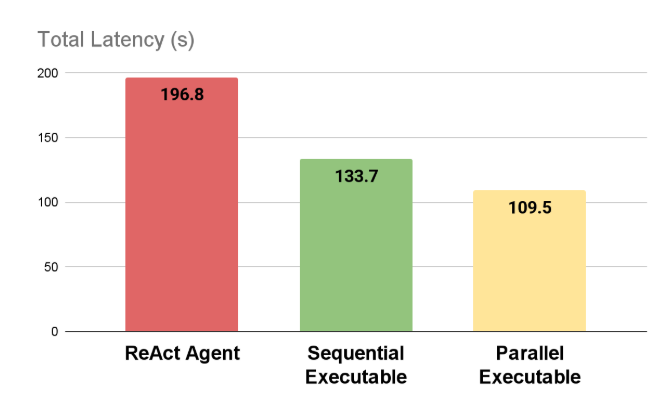
\includegraphics[scale=0.5]{images/latency.png}
\caption{Latency Performance Across 12 Test Cases}
\label{fig:latency_comparison_ch4}
\end{figure}

As shown in Figure~\ref{fig:latency_comparison_ch4}, the latency profile favors the fully parallel executable agent, which completed the suite roughly 20–25\% faster than the sequential counterpart. However, latency alone is not decisive for IDE scenarios, where reliability under load is equally critical.

\begin{figure}[H]
\centering
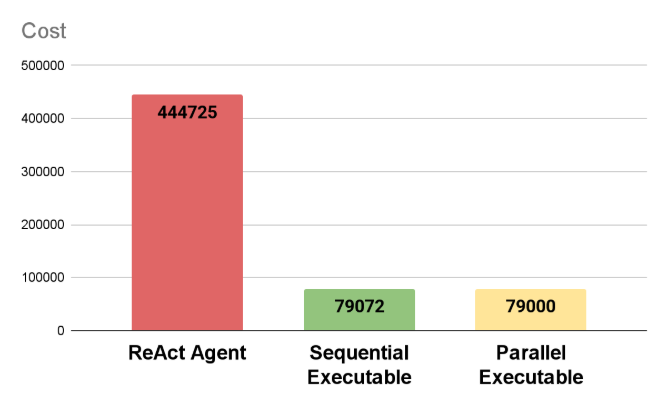
\includegraphics[scale=0.5]{images/cost.png}
\caption{Cost Analysis Across 12 Test Cases}
\label{fig:cost_comparison_ch4}
\end{figure}

As shown in Figure~\ref{fig:cost_comparison_ch4}, token cost highlights a fundamental inefficiency in the ReAct agent: due to iterative reasoning–acting loops, it consumes orders of magnitude more tokens (≈6x in our suite) to achieve comparable outcomes. This renders ReAct non‑viable for an interactive IDE use case.

\begin{figure}[H]
\centering
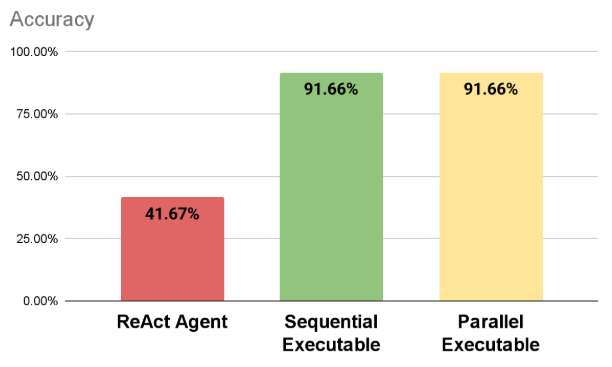
\includegraphics[scale=0.5]{images/accuracy.png}
\caption{Accuracy Performance Across 12 Test Cases}
\label{fig:accuracy_comparison_ch4}
\end{figure}

As shown in Figure~\ref{fig:accuracy_comparison_ch4}, both executable variants achieved high accuracy (Sequential at ≈91.7\%, Parallel matching on successful runs). Yet, the apparent parity masks a practical limitation: under heavier workloads, the fully parallel strategy occasionally failed with resource‑limit and deadline errors. In an IDE, such instability outweighs raw speed advantages.\\

Synthesizing these findings, we adopted a \textbf{Parallel Executable architecture with bounded concurrency}. By enforcing semaphore‑based limits on in‑flight LLM calls, the design retains most of the latency advantage of full parallelism while eliminating overload‑induced failures. This yields a deterministic, high‑throughput, and reliable execution profile appropriate for production IDE integration.

\subsubsection{Agent Implementation Overview}
The AI Agent implements the chosen architecture using Python and integrates with Google’s internal AI platform 
hosting Gemini-based LLMs. The design is class-based and modular, ensuring extensibility, observability, and testability.  
The agent exposes a single \texttt{execute()} entry point, orchestrating a pipeline of specialized tools that handle 
file reading, analysis, explanation generation, fix generation, and result consolidation.

\paragraph{Configuration and Initialization}
At startup, the agent performs several critical setup tasks:
\begin{itemize}
    \item \textbf{Model Selection:} Configured to use the latest Gemini-based model trained on internal Google code.
    \item \textbf{Convention Loading:} Best practices are defined as in-memory Python objects and loaded at startup into a cache for constant-time access.
    \item \textbf{Tool Registration:} The five specialized tools are instantiated and registered into a deterministic workflow.
\end{itemize}

\paragraph{Implementation Structure}
The implementation follows a layered orchestration pattern:
\begin{itemize}
    \item A central agent class orchestrates the pipeline via dependency-injected tools.
    \item Each tool is encapsulated as a class with clear \texttt{run()} contracts and typed inputs/outputs.
    \item Metrics and token usage are logged per tool, enabling fine-grained observability.
    \item Separation of concerns allows tools to be replaced or extended without modifying orchestration logic.
\end{itemize}

\subsubsection{Core Tools Implementation}
The agent implements five specialized tools, each corresponding to one stage of the analysis pipeline. Tools are designed as independent classes that expose a public \texttt{run()} method, which enforces a clear input/output contract and raises typed errors when failures occur. This contract-based design makes the system modular, testable, and resilient to partial failures.

\paragraph{ReadFileFromWorkspace Tool}\\
\textbf{Contract:} input = file path; output = file content (string).  
The ReadFileFromWorkspace tool is responsible for retrieving the contents of the developer’s source file. Implementation details include:
\begin{itemize}
    \item \textbf{File system access:} Uses Python’s built-in file handling with UTF-8 as the default encoding, while detecting and recovering from alternative encodings.
    \item \textbf{Error handling:} Raises typed errors such as \texttt{FileNotFoundError}, \texttt{PermissionDeniedError}, and \texttt{EncodingError}. These errors are logged and surfaced to the developer in structured form.
    \item \textbf{Robustness:} Handles large files by streaming content, ensuring memory efficiency.
\end{itemize}

\paragraph{CodeAnalysisTool}\\
\textbf{Contract:} input = file content; output = list of base violations.  
This tool forms the analysis core of the system. It detects framework violations by orchestrating LLM queries enriched with contextual information.
\begin{itemize}
    \item \textbf{Prompt construction:} Implements a template system with slots for file type, code snippet, and dynamically filtered convention definitions.
    \item \textbf{Context injection:} Selects relevant conventions from the cache and injects them into the prompt to guide the model.
    \item \textbf{Response parsing:} Uses strict schema validation with recovery mechanisms for malformed LLM responses.
    \item \textbf{Performance optimizations:} Employs caching of templates and convention definitions, reducing repeated token usage and lowering latency.
\end{itemize}

\paragraph{ViolationExplanationTool}\\
\textbf{Contract:} input = base violation; output = natural-language explanation.  
The ViolationExplanationTool generates educational explanations that help developers understand not only what the violation is, but why it matters.
\begin{itemize}
    \item \textbf{Contextualization:} Pulls in violation metadata (rule violated, line number, code snippet) to ground explanations in concrete evidence.
    \item \textbf{Generation style:} Prompts the LLM to balance technical accuracy with readability, avoiding overly generic statements.
    \item \textbf{Implementation detail:} Each explanation is post-processed for clarity, removing redundant phrasing and enforcing concise output.
\end{itemize}

\paragraph{CodeFixTool}\\
\textbf{Contract:} input = violation + explanation; output = code fix (annotated snippet).  
This tool provides actionable, safe, and educational fixes.
\begin{itemize}
    \item \textbf{Safety:} Fixes are constrained to local code changes, avoiding edits that break APIs or dependencies.
    \item \textbf{Self-containment:} Ensures that each fix can be applied without requiring modifications in other files.
    \item \textbf{Contextual adaptation:} Uses file content and violation metadata to adapt fixes to the surrounding code style.
    \item \textbf{Educational emphasis:} Each fix includes explanatory comments describing why the change is required.
    \item \textbf{Error handling:} Raises a \texttt{FixGenerationError} if the LLM output cannot be parsed or validated as compilable code.
\end{itemize}

\paragraph{Finish Tool}\\
\textbf{Contract:} input = violations + explanations + fixes; output = structured response for IDE extension.  
The Finish Tool acts as the consolidation component, producing a structured JSON response that the IDE extension can directly render.
\begin{itemize}
    \item \textbf{Aggregation:} Combines violations, explanations, and fixes into a unified structure keyed by violation ID.
    \item \textbf{Deduplication:} Identifies overlapping or redundant violations and merges them to reduce noise.
    \item \textbf{Validation:} Ensures schema compliance so that the IDE can reliably parse and render results.
    \item \textbf{Formatting:} Applies consistent formatting (line numbers, code blocks, explanations) to improve readability in the UI.
\end{itemize}

\noindent Collectively, these tools form a deterministic pipeline coordinated by the agent’s \texttt{execute()} method. Each tool adheres to explicit contracts, which improves modularity, observability (per-tool token usage is logged), and long-term maintainability.


\subsubsection{Processing Workflow}

\begin{figure}[H]
    \centering
    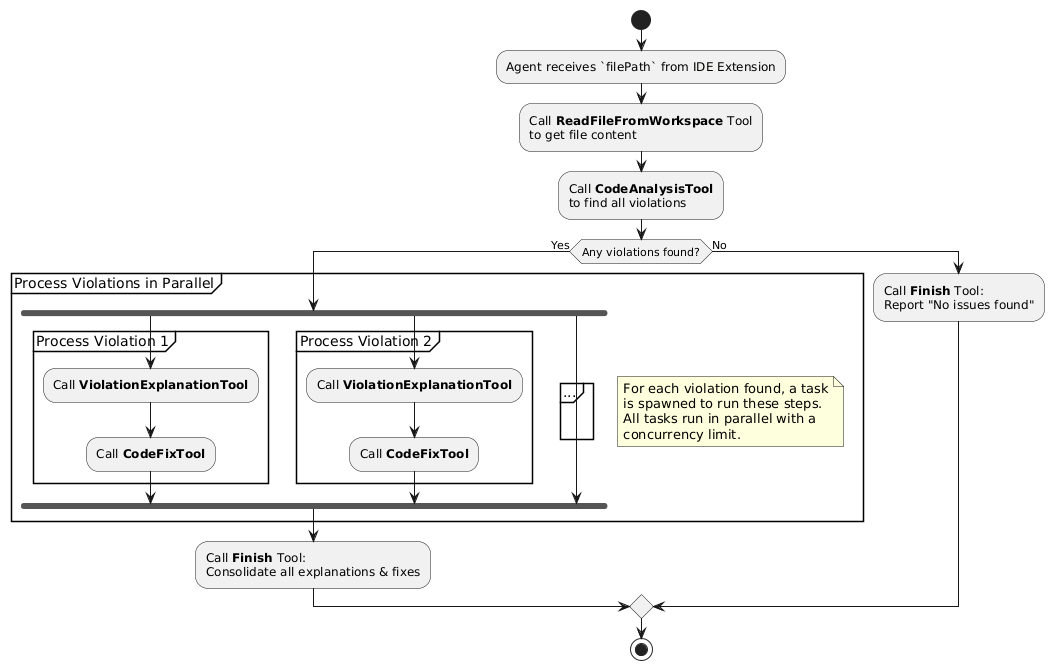
\includegraphics[scale=0.5]{images/activity_diagram.png}
    \caption{Agent Processing Activity Diagram}
    \label{fig:agent_activity}
\end{figure}

As illustrated in the activity diagram in figure~\ref{fig:agent_activity}, the hybrid strategy is realized in three main stages:
\begin{enumerate}
    \item \textbf{Sequential Preprocessing:} Full file content is read and all violations are identified.
    \item \textbf{Parallel Processing:} Explanation and fix generation tasks are executed concurrently with semaphore-based 
    limits on in-flight LLM calls.
    \item \textbf{Result Consolidation:} Outputs are aggregated, validated, and prepared for the IDE extension.
\end{enumerate}



\subsubsection{Resilience and Error Handling}
The system ensures graceful degradation under failures:
\begin{itemize}
    \item Independent processing of violations isolates failures to individual tasks.
    \item Retry with exponential backoff mitigates transient network or LLM errors.
    \item Typed error classes facilitate debugging and developer support.
    \item Partial results are preserved, ensuring developers always receive usable feedback.
\end{itemize}

\subsubsection{Convention Data Management}
The convention data management system implements loading, caching, and retrieval mechanisms for YouTube framework best practices. The conventions are stored as Python objects in an array, each containing a unique identifier, description, correct example, and incorrect example. For efficient runtime access, the system constructs an \textbf{in-memory map} keyed by convention ID, allowing the agent tools to retrieve only the relevant convention on demand. 

\paragraph{Loading and Initialization}
At startup, all convention objects are loaded into memory from the Python array. A dictionary (map) is created with convention IDs as keys and convention objects as values, providing constant-time access for subsequent tool invocations.

\paragraph{Memory Caching and Access}
This in-memory caching strategy ensures low-latency access during code analysis:

\begin{itemize}
    \item \textbf{Efficient Lookup}: Tools retrieve conventions by ID from the map, avoiding iteration over the full array.
    \item \textbf{Dynamic Selection}: Only conventions relevant to the current file type and analysis context are queried, minimizing unnecessary data processing.
    \item \textbf{Lightweight and Fast}: The cache resides entirely in memory, requiring no external services, and supports rapid retrieval during concurrent tool executions.
\end{itemize}

\subsection{Extension Integration}

\subsubsection{Extension Architecture}
The IDE Extension implements a layered architecture that integrates with the overall system through three distinct layers: the Extension layer containing user-facing components, a Proxy layer for authentication and request routing, and the Backend layer hosting AI agent services.

\begin{figure}[H]
    \centering
    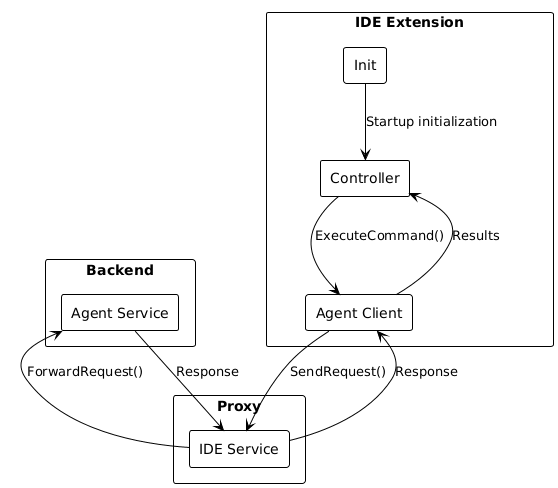
\includegraphics[scale=0.6]{Images/extension_integration.png}
    \caption{System Architecture: IDE Extension, Proxy, and Backend Communication Flow}
    \label{fig:high_level_frontend_architecture}
\end{figure}

The architecture follows a clear request-response pattern where user interactions trigger analysis requests that flow through the IDE Service proxy for authentication and authorization, then to the Agent Service in the backend for processing. Responses follow the same path in reverse, ensuring secure and authenticated communication throughout the entire pipeline while maintaining clear separation of responsibilities between layers.

\paragraph{Extension Components}
The extension's internal architecture consists of three core components that work together to provide seamless integration with the development environment, as illustrated in Figure~\ref{fig:high_level_frontend_architecture}.

\textbf{Init Component}: Handles extension initialization, reading user settings, registering commands and editor actions, and performing health checks. The component ensures proper setup of all dependencies.

\textbf{Controller}: Centralizes all UI-related state and orchestrates interactions between components. The Controller processes commands, manages notifications, routes analysis results, renders diagnostics and hover-based suggestions, and coordinates stale-state transitions to ensure consistent behavior across all entry points.

\textbf{AgentClient}: Manages communication with the backend services through the proxy layer. The component handles request formatting, implements retry logic with exponential backoff, manages timeouts, and processes responses from the AI agent.

\subsubsection{User Interaction}
The feature is controlled through a dedicated \textbf{user setting}. This setting appears as a simple checkbox: when enabled, the feature becomes available in the IDE; when disabled, it is entirely hidden from the interface. This ensures that developers can opt in seamlessly without cluttering the environment for those who do not use the feature.

The primary entry point for triggering analysis is an \textbf{Editor Action} integrated into the file title bar (Figure~\ref{fig:editor_action_implementation}). This placement ensures high visibility and aligns naturally with the developer’s workflow when working on individual files.

\begin{figure}[H]
    \centering
    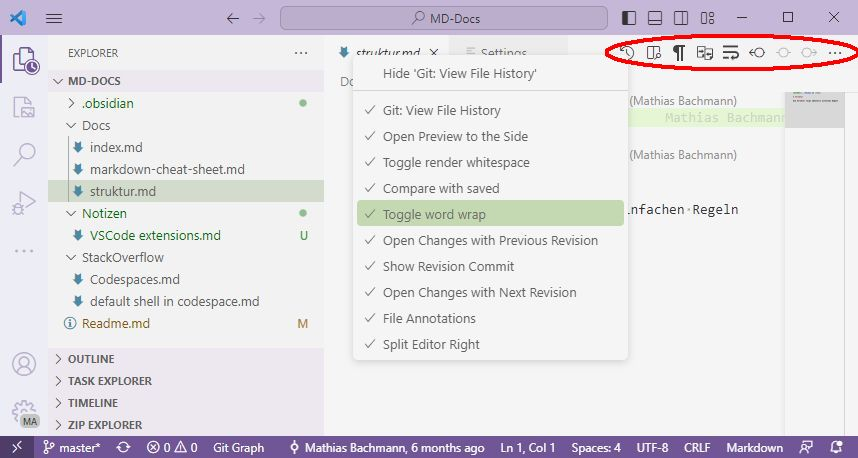
\includegraphics[scale=0.4]{Images/editor_actions.jpg}
    \caption{VS Code Interface: Editor Actions (Illustrative).}
    \label{fig:editor_action_implementation}
\end{figure}

An additional entry point is provided through the \textbf{Command Palette}, which can be invoked using \texttt{Ctrl+Shift+P} (or \texttt{Cmd+Shift+P} on macOS). This pathway makes the feature equally accessible to developers who prefer keyboard-driven workflows and ensures discoverability for new users exploring available commands (Figure~\ref{fig:command_palette_example}).

\begin{figure}[H]
    \centering
    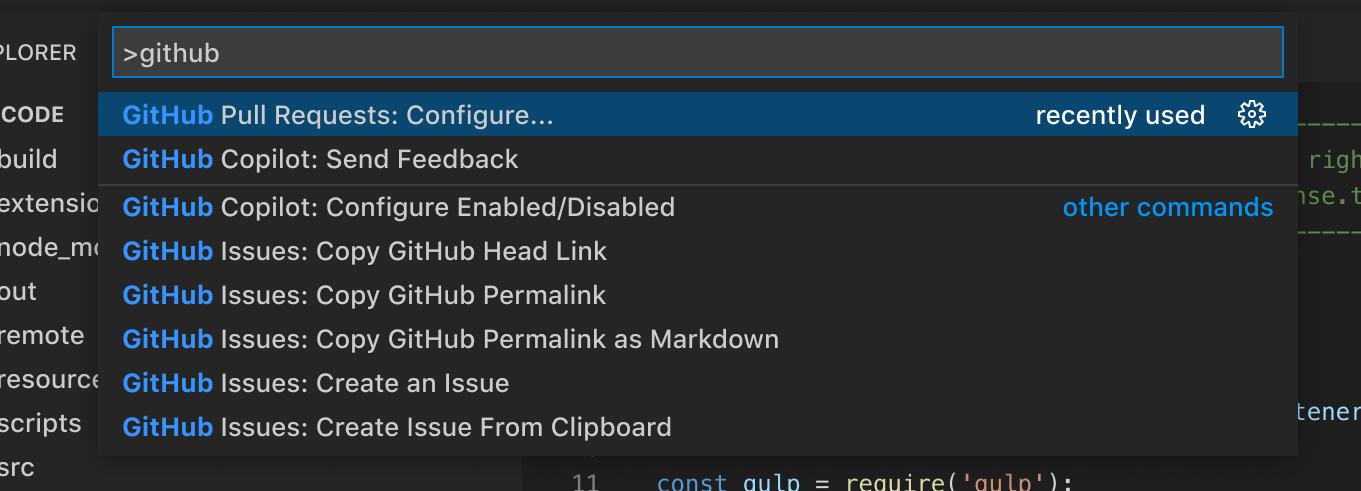
\includegraphics[scale=0.5]{Images/command_palette.png}
    \caption{VS Code Command Palette (Illustrative).}
    \label{fig:command_palette_example}
\end{figure}


Once analysis is triggered, the extension provides immediate feedback via \textbf{VS Code notifications} (Figure~\ref{fig:notification_example}). These notifications confirm that a request has been received, update progress, and display clear error messages if issues occur. This ensures transparent communication throughout the request lifecycle.

\begin{figure}[H]
    \centering
    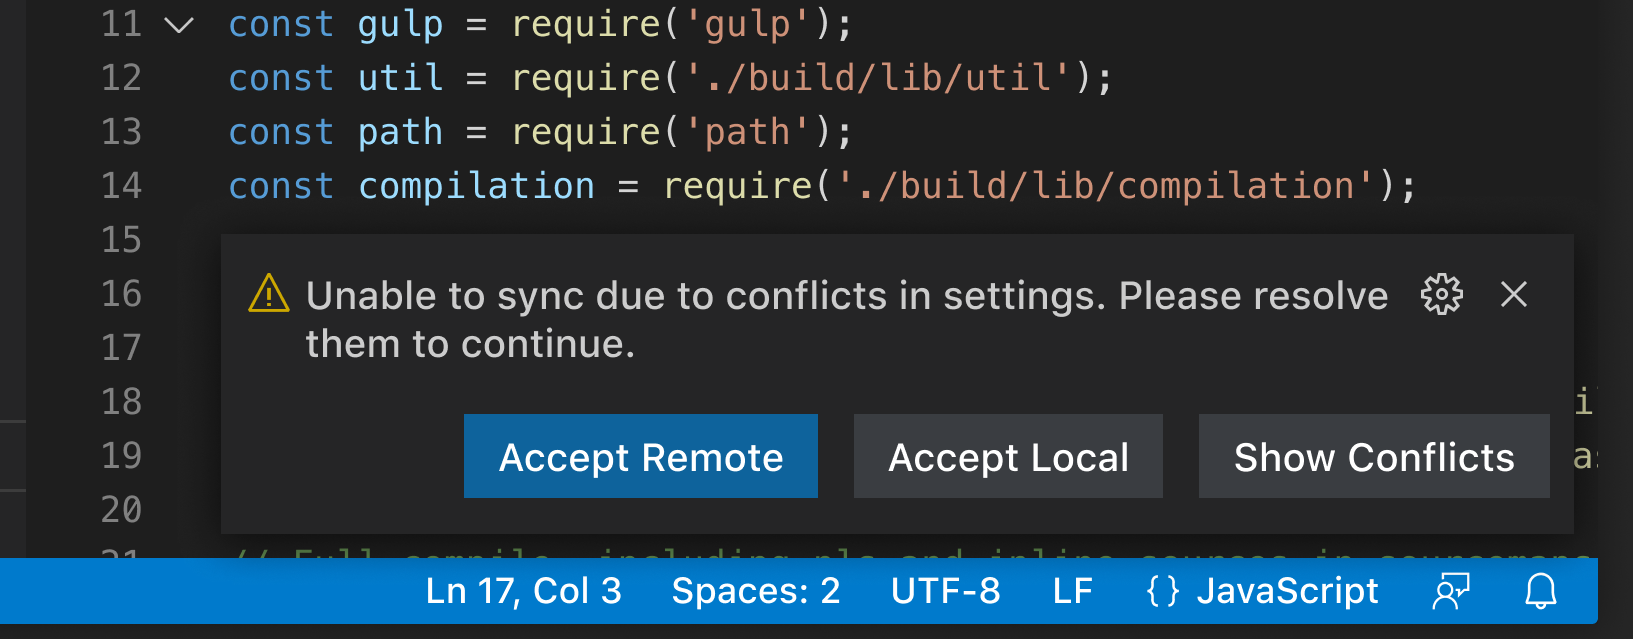
\includegraphics[scale=0.8]{Images/vscode_notification.png}
    \caption{VS Code Notification Interface (Illustrative).}
    \label{fig:notification_example}
\end{figure}

The results of the analysis are surfaced through VS Code’s native \textbf{diagnostic system}. Violations appear in the \textbf{Problems panel} and are underlined directly in the editor, marking the exact range of code that violates a best practice (Figure~\ref{fig:diagnostics_example}). Hovering over the highlighted code reveals the diagnostic explanation, helping developers quickly understand the issue in context.

\begin{figure}[H]
    \centering
    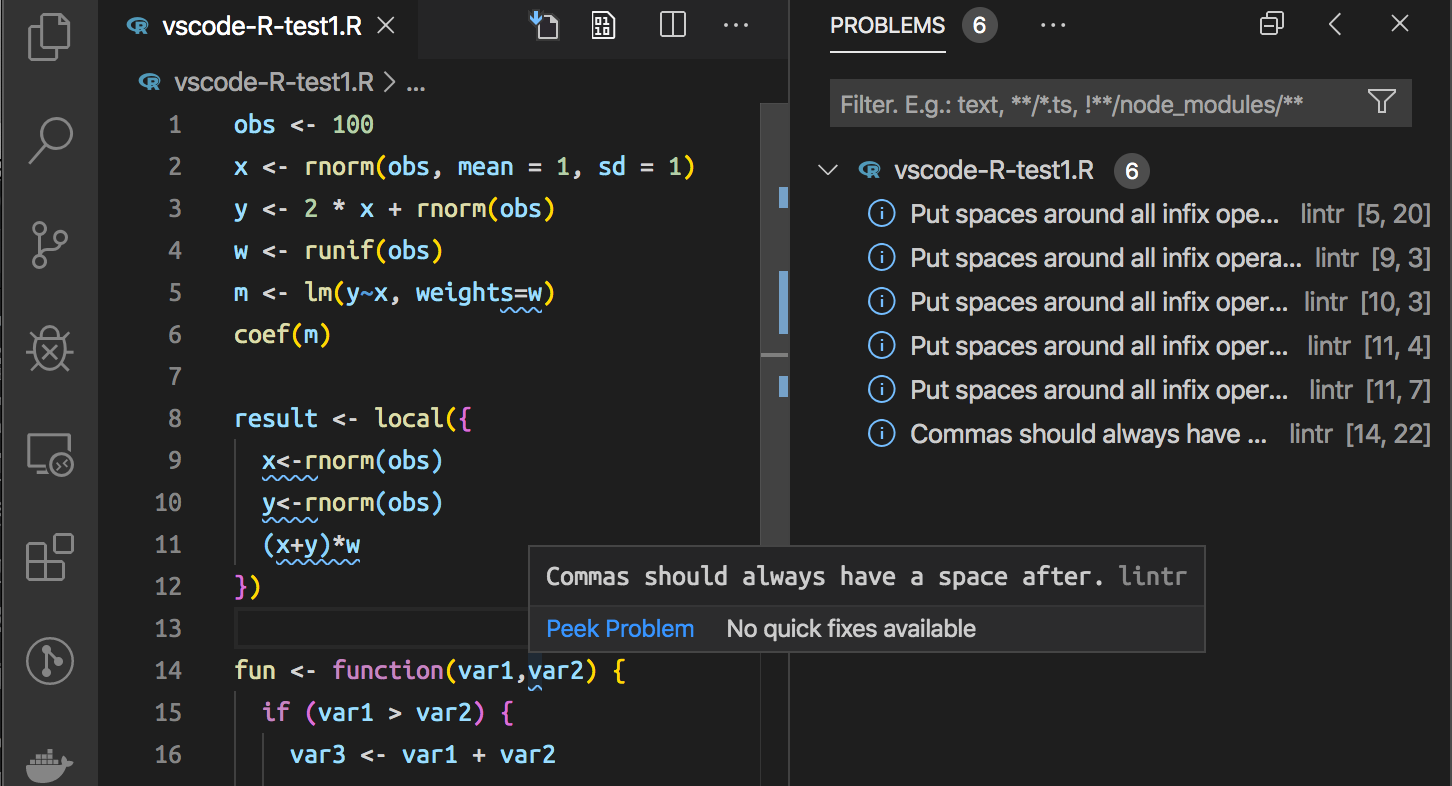
\includegraphics[scale=0.4]{Images/vscode_diagnostics.png}
    \caption{VS Code Diagnostics Interface (Illustrative).}
    \label{fig:diagnostics_example}
\end{figure}

For more detailed guidance, an integrated \textbf{hover provider} presents formatted fix suggestions directly within the editor. This approach allows fixes to be displayed with proper syntax highlighting and inline code snippets, offering a clear and actionable path to resolution without leaving the development workflow.

\subsubsection{Stale Diagnostics Handling}
One of the most challenging aspects of IDE integration is maintaining diagnostic accuracy as developers continuously modify their code. The extension implements a sophisticated two-tiered system that balances immediate responsiveness with accurate analysis results.

\paragraph{The Challenge}
Traditional diagnostic systems struggle with code that changes rapidly, often displaying outdated information that confuses developers and reduces trust in the tool. The challenge is to provide immediate visual feedback while ensuring that diagnostics remain accurate and relevant to the current code state.

\paragraph{Two-Tiered Solution}  
The extension handles stale diagnostics using a two-tiered approach that separates immediate responsiveness from precise re-anchoring:  

\textbf{Tier 1 - Instant Adjustment}: Provides immediate feedback on every keystroke. Diagnostics are shifted based on simple text edits and marked as [Outdated] if the flagged code itself is edited. This ensures high \textbf{responsiveness} without impacting performance.  

\textbf{Tier 2 - Debounced Re-anchoring}: Activates after a 1-second pause in typing to improve diagnostic \textbf{accuracy}. The process involves:  
\begin{enumerate}
    \item \textbf{Fingerprint}: Creates a contextual hash from the code and its surrounding context to identify exact matches.  
    \item \textbf{Scan with Regex}: Finds all possible text matches across the document.  
    \item \textbf{Re-anchor}: Moves the diagnostic to the correct new location based on the highest match score.  
\end{enumerate}  
This two-tiered strategy balances responsiveness with accuracy, ensuring developers receive timely feedback while maintaining the integrity of diagnostics even during active code editing.


\begin{figure}[H]
    \centering
    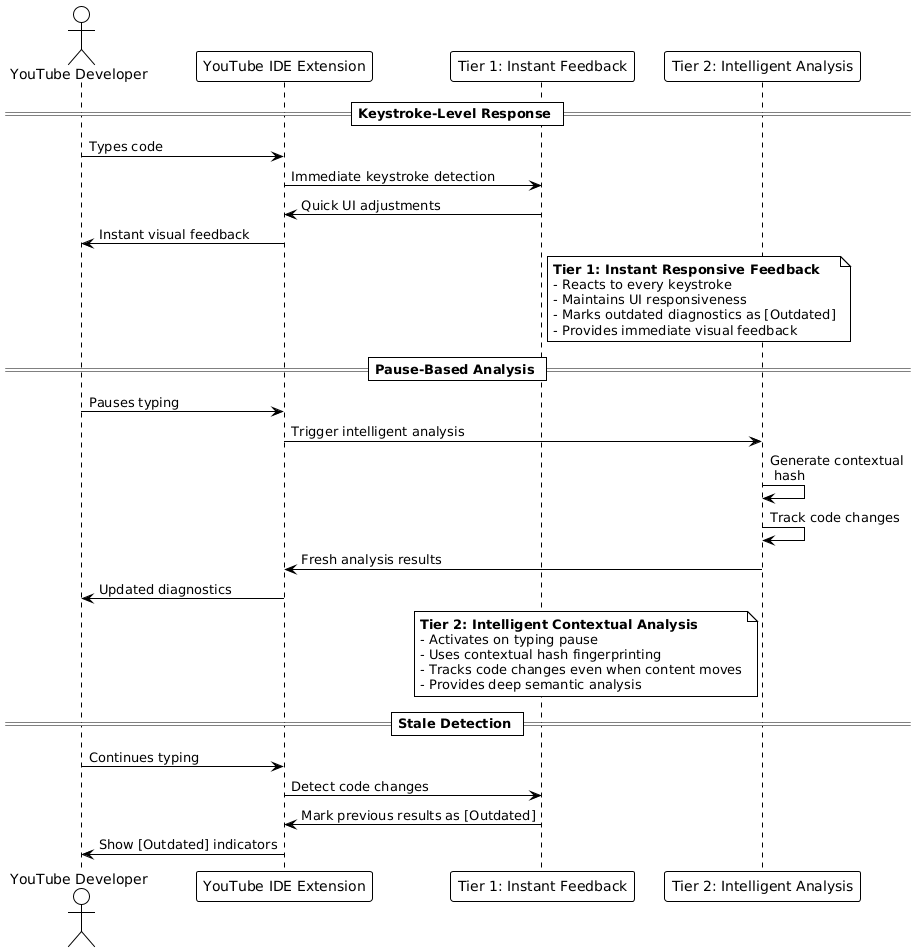
\includegraphics[scale=0.55]{Images/stale_diagnostics.png}
    \caption{Stale Diagnostics Handling: Two-Tiered System (Illustrative)}
    \label{fig:stale_diagnostics_method}
\end{figure}

This approach ensures that developers receive immediate visual feedback while maintaining diagnostic accuracy through intelligent analysis timing and state management, representing a significant technical contribution to IDE integration challenges.

\subsubsection{Resilience and Communication}
The extension implements comprehensive error handling and resilience mechanisms to ensure reliable operation in production environments. The communication system uses internal RPC infrastructure with JSON payloads for debugging and cross-language compatibility.

Error handling follows fault-tolerant design principles with multi-level error isolation, ensuring that failures in one component do not cascade to others. The system implements specific error types for different failure scenarios, including network communication errors, service unavailability, and timeout errors, with detailed error information and suggested recovery actions.

Retry mechanisms with exponential backoff and bounded attempts ensure operation under transient failure conditions, while timeout management prevents indefinite waiting periods and maintains responsive user experience. The implementation includes request validation and response parsing to prevent communication errors and ensure data integrity throughout the analysis pipeline.


\section*{Conclusion}
This chapter presented the evaluation results, the resulting architecture decision (Parallel Executable with concurrency limiting), and the complete implementation: environment, technologies, and realization across backend and IDE. The system is production-oriented, balancing speed with stability and cost.

%==============================================================================
\end{spacing}